\documentclass[10pt,aspectratio=169]{beamer}

% --- Theme: clean default look, matching deck_theme_discovery style ---
\usetheme{default}
\setbeamertemplate{navigation symbols}{}
\setbeamertemplate{footline}{%
  \hfill\insertframenumber/\inserttotalframenumber\hspace{1em}\vspace{0.4em}}
\setbeamercolor{title}{fg=black}
\setbeamercolor{frametitle}{fg=black}
\setbeamerfont{frametitle}{series=\bfseries}
\setbeamerfont{title}{series=\bfseries, size=\Large}

% --- Packages ---
\usepackage[utf8]{inputenc}
\usepackage[T1]{fontenc}
\usepackage{graphicx}
\usepackage{booktabs}
\usepackage{tikz}
\usetikzlibrary{shapes.geometric, arrows.meta, positioning, calc}
\usepackage{xcolor}
\usepackage{amsmath}
\usepackage{amssymb}
\usepackage{tcolorbox}
\tcbuselibrary{skins}

% --- Corporate-ish palette (matches the reference Intesa-style slide) ---
\definecolor{corpblue}{RGB}{15, 56, 122}
\definecolor{corpgreen}{RGB}{30, 110, 60}
\definecolor{corporange}{RGB}{220, 130, 30}
\definecolor{corplight}{RGB}{220, 230, 245}

% --- Tableau-ish accents (consistent with deck1/deck2) ---
\definecolor{good}{RGB}{44,160,44}
\definecolor{bad}{RGB}{214,39,40}
\definecolor{warn}{RGB}{255,140,0}
\definecolor{accent}{RGB}{31,119,180}

% --- Section break helper ---
\newcommand{\mybreak}[1]{%
  \begin{frame}[plain]
    \centering
    \vspace*{\fill}
    {\LARGE\bfseries #1}
    \vspace*{\fill}
  \end{frame}}

% --- Corporate-style header panel for slide 2 ---
\newcommand{\panelheader}[3]{% color, title, subtitle
  \begin{tcolorbox}[
      enhanced, colback=#1, colframe=#1,
      boxrule=0pt, arc=2pt, left=10pt, right=10pt, top=6pt, bottom=6pt,
      sharp corners=southwest]
    {\color{white}\bfseries\large #2}\\[0.05cm]
    {\color{corporange}\scriptsize\bfseries\textsc{#3}}
  \end{tcolorbox}}

\title{Theme Discovery --- Overview}
\subtitle{Objective, taxonomy, definition, current pipeline}
\date{May 2026}

\begin{document}

% =====================================================================
% Title
% =====================================================================
\begin{frame}[plain]
  \titlepage
  \vspace{-0.6cm}
  \centering\small
  \emph{One deck, four ideas: where this fits, what we mean by ``theme'',
  and what the pipeline looks like today.}
\end{frame}


% =====================================================================
% Why thematic trading? - the motivation
% =====================================================================
\begin{frame}{Why thematic trading?}
  \footnotesize

  \textbf{Traditional sector investing} organises companies along
  \emph{time-invariant} axes --- sector, geography, market cap, style.
  \begin{itemize}\setlength\itemsep{0.04cm}
    \item Easy to benchmark, easy to index.
    \item Slow to capture structural shifts that cut \emph{across} sectors.
  \end{itemize}

  \vspace{0.30cm}
  \textbf{Thematic trading} organises companies along a \emph{narrative} ---
  a structural change driving demand across multiple sectors at once.
  \begin{itemize}\setlength\itemsep{0.04cm}
    \item \textbf{AI infrastructure} $\rightarrow$ chip designers + utilities + cooling + real estate
    \item \textbf{Energy transition} $\rightarrow$ miners + grid operators + auto manufacturers
    \item \textbf{GLP-1 obesity drugs} $\rightarrow$ pharma + food \& beverage + medical devices
  \end{itemize}

  \vspace{0.30cm}
  \begin{tcolorbox}[colback=corplight, colframe=corplight,
                    boxrule=0pt, arc=2pt,
                    left=10pt, right=10pt, top=5pt, bottom=5pt]
    \centering\footnotesize
    \textbf{The bet:} catch the narrative \emph{before} it is priced into every constituent.
  \end{tcolorbox}

\end{frame}


% =====================================================================
% Objective - corporate two-panel layout
% =====================================================================
\begin{frame}{AI-Powered Thematic Alpha --- where this work fits}
  \footnotesize

  \begin{columns}[T,onlytextwidth]
    \column{0.49\textwidth}
      \panelheader{corpblue}{AI Thematic Detection}{extracting alpha}
      \vspace{0.10cm}
      \begin{itemize}\setlength\itemsep{0.10cm}
        \item Monitor \textbf{news, social media, podcasts,
              prediction markets} and other real-time sources
              to surface emerging themes \emph{before consensus}.
        \item Detect \textbf{acceleration and inflection points}
              in attention/sentiment around predefined themes.
        \item \textbf{Unsupervised discovery} of new investment themes
              from the corpus.
      \end{itemize}
      \vspace{0.10cm}
      \textbf{\textcolor{corpblue}{$\blacktriangleleft$ Focus of this deck.}}

    \column{0.49\textwidth}
      \panelheader{corpgreen}{AI Basket Construction}{trade implementation}
      \vspace{0.10cm}
      \begin{itemize}\setlength\itemsep{0.10cm}
        \item AI-driven \textbf{thematic baskets} with dynamic
              rebalancing.
        \item \textbf{On-demand portfolio construction} from
              natural-language prompts.
        \item AI-based mapping of \textbf{companies, suppliers, and
              value-chain relationships} (supply risk, second-order
              exposure).
      \end{itemize}
      \vspace{0.10cm}
      \textbf{\textcolor{corpgreen}{Next leg, downstream of detection.}}
  \end{columns}

  \vspace{0.20cm}
  \begin{tcolorbox}[colback=corplight, colframe=corplight,
                    boxrule=0pt, arc=2pt, left=8pt, right=8pt, top=4pt, bottom=4pt]
    \footnotesize
    \textbf{Product outcomes:}\;
    Alpha signals \quad\textbullet\quad
    Investing in emerging topics \quad\textbullet\quad
    Thematic baskets
  \end{tcolorbox}

\end{frame}


% =====================================================================
% Taxonomy - granularity ladder + sectors
% =====================================================================
\begin{frame}{Taxonomy --- how we organise the world}
  \footnotesize

  \textbf{Granularity ladder.}\;
  News carries events; events recur into themes; themes plus exposure
  become tradable.

  \vspace{0.10cm}
  \begin{center}
  \resizebox{0.97\textwidth}{!}{%
  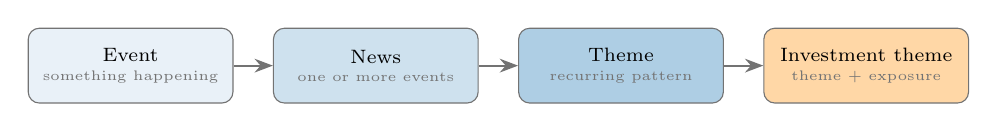
\begin{tikzpicture}[
      node distance=0.1cm,
      box/.style={rectangle, rounded corners, draw=black!55, line width=0.4pt,
                  minimum width=2.6cm, minimum height=0.95cm,
                  font=\scriptsize, align=center},
      arr/.style={-Stealth, thick, draw=black!55}
    ]
    \node[box, fill=accent!10] (e) {Event\\[-0.05cm]\textcolor{black!55}{\tiny something happening}};
    \node[box, fill=accent!22, right=0.50cm of e] (n) {News\\[-0.05cm]\textcolor{black!55}{\tiny one or more events}};
    \node[box, fill=accent!36, right=0.50cm of n] (t) {Theme\\[-0.05cm]\textcolor{black!55}{\tiny recurring pattern}};
    \node[box, fill=warn!35,   right=0.50cm of t] (i) {Investment theme\\[-0.05cm]\textcolor{black!55}{\tiny theme + exposure}};
    \draw[arr] (e) -- (n);
    \draw[arr] (n) -- (t);
    \draw[arr] (t) -- (i);
  \end{tikzpicture}}
  \end{center}

  \vspace{0.20cm}
  \textbf{Sectors --- the time-invariant baseline.}\;
  Several taxonomies exist; companies' sector codes rarely change.

  \vspace{0.10cm}
  \begin{center}
  \begin{tabular}{@{}lll@{}}
    \toprule
    Standard & Maintained by & Granularity \\
    \midrule
    \textbf{GICS}  & MSCI / S\&P    & 11 sectors $\rightarrow$ 25 industry groups $\rightarrow$ 74 industries \\
    \textbf{ICB}   & FTSE Russell   & 11 industries $\rightarrow$ 20 supersectors $\rightarrow$ 45 sectors \\
    \textbf{RBICS} & FactSet        & $\sim$1{,}500 leaf-level sub-industries (revenue-based) \\
    \bottomrule
  \end{tabular}
  \end{center}

  \vspace{0.15cm}
  \textit{What sectors cannot capture:} cross-sector narratives, transient
  shifts, and firms whose \textbf{thematic exposure is much larger than
  their sector classification suggests.}

\end{frame}


% =====================================================================
% Theme definition + Clean Energy example
% =====================================================================
\begin{frame}{What is a theme? --- definition + Clean Energy example}
  \footnotesize

  \begin{columns}[T,onlytextwidth]
    \column{0.40\textwidth}
      \begin{tcolorbox}[colback=corpblue!8, colframe=corpblue,
                        boxrule=0.4pt, arc=2pt,
                        left=6pt, right=6pt, top=4pt, bottom=4pt]
        \footnotesize
        \textbf{Theme} = a coherent narrative tying together a stream of events.
        Two defining properties:
        \begin{enumerate}\setlength\itemsep{0.04cm}
          \item \textbf{Transient} --- has a lifecycle (emerge,
                accelerate, mature, fade).
          \item \textbf{Cross-sector} --- groups firms a sector
                taxonomy would scatter.
        \end{enumerate}
      \end{tcolorbox}

      \vspace{0.15cm}
      \textbf{Operational definition for this project:}\;
      a cluster of events that recur together over a sustained window
      and are mentioned in news with rising frequency.

    \column{0.59\textwidth}
      \textbf{Example --- Clean Energy 2018--2024.}

      \vspace{0.10cm}
      \emph{Cross-sector by construction.}
      One narrative, beneficiaries in five different GICS sectors:
      utilities (NEE), industrials (ENPH, VWS), materials (ALB),
      autos (TSLA), tech (solar inverters, grid software).

      \vspace{0.20cm}
      \emph{Lifecycle, in one line per stage:}
      \begin{center}
      \resizebox{0.98\textwidth}{!}{%
      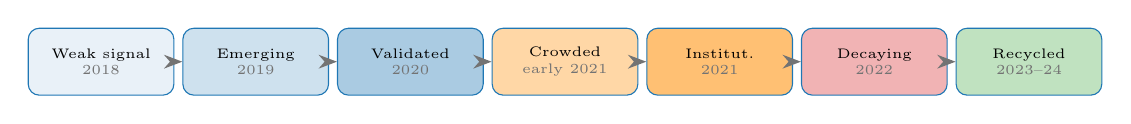
\begin{tikzpicture}[
          node distance=0.05cm,
          stage/.style={rectangle, rounded corners, draw=accent, line width=0.4pt,
                        minimum width=1.85cm, minimum height=0.85cm,
                        font=\tiny, align=center},
          arr/.style={-Stealth, thick, draw=black!55}
        ]
        \node[stage, fill=accent!10] (a) {Weak signal\\\textcolor{black!55}{2018}};
        \node[stage, fill=accent!22, right=0.10cm of a] (b) {Emerging\\\textcolor{black!55}{2019}};
        \node[stage, fill=accent!38, right=0.10cm of b] (c) {Validated\\\textcolor{black!55}{2020}};
        \node[stage, fill=warn!35,   right=0.10cm of c] (d) {Crowded\\\textcolor{black!55}{early 2021}};
        \node[stage, fill=warn!55,   right=0.10cm of d] (e2) {Institut.\\\textcolor{black!55}{2021}};
        \node[stage, fill=bad!35,    right=0.10cm of e2] (f) {Decaying\\\textcolor{black!55}{2022}};
        \node[stage, fill=good!30,   right=0.10cm of f] (g) {Recycled\\\textcolor{black!55}{2023--24}};
        \draw[arr] (a) -- (b);
        \draw[arr] (b) -- (c);
        \draw[arr] (c) -- (d);
        \draw[arr] (d) -- (e2);
        \draw[arr] (e2) -- (f);
        \draw[arr] (f) -- (g);
      \end{tikzpicture}}
      \end{center}

      \vspace{0.05cm}
      \emph{What the trade was worth.}\;
      ICLN: $\sim\$10$ early 2020 $\rightarrow$ $\sim\$33$ Jan 2021 ($\sim$3.3$\times$).
      Most of the return happened in the \textbf{emerging $\rightarrow$ crowded}
      window (2019--early 2021). By the time the trade was institutionalised,
      it was over.

  \end{columns}

\end{frame}


% =====================================================================
% Current pipeline - high level
% =====================================================================
\begin{frame}{The pipeline today --- high-level view}
  \footnotesize

  \begin{center}
  \resizebox{0.97\textwidth}{!}{%
  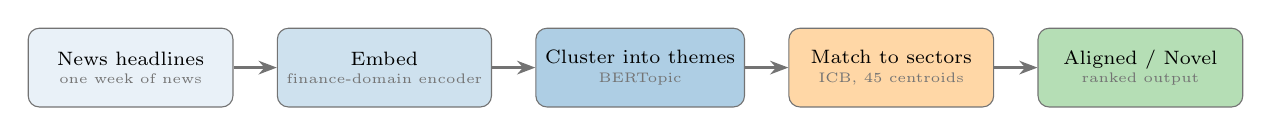
\begin{tikzpicture}[
      node distance=0.1cm,
      box/.style={rectangle, rounded corners, draw=black!55, line width=0.4pt,
                  minimum width=2.6cm, minimum height=1.0cm,
                  font=\scriptsize, align=center},
      arr/.style={-Stealth, thick, draw=black!55}
    ]
    \node[box, fill=accent!10] (n) {News headlines\\[-0.05cm]\textcolor{black!55}{\tiny one week of news}};
    \node[box, fill=accent!22, right=0.55cm of n] (e) {Embed\\[-0.05cm]\textcolor{black!55}{\tiny finance-domain encoder}};
    \node[box, fill=accent!36, right=0.55cm of e] (c) {Cluster into themes\\[-0.05cm]\textcolor{black!55}{\tiny BERTopic}};
    \node[box, fill=warn!35,   right=0.55cm of c] (m) {Match to sectors\\[-0.05cm]\textcolor{black!55}{\tiny ICB, 45 centroids}};
    \node[box, fill=good!35,   right=0.55cm of m] (o) {Aligned / Novel\\[-0.05cm]\textcolor{black!55}{\tiny ranked output}};
    \draw[arr] (n) -- (e);
    \draw[arr] (e) -- (c);
    \draw[arr] (c) -- (m);
    \draw[arr] (m) -- (o);
  \end{tikzpicture}}
  \end{center}

  \vspace{0.20cm}
  \begin{columns}[T,onlytextwidth]
    \column{0.49\textwidth}
      \textbf{What it produces.}
      \begin{itemize}\setlength\itemsep{0.04cm}
        \item A short list of themes, each tagged with the
              \textbf{nearest sector} and a similarity score.
        \item Two buckets: \emph{aligned} (the theme fits a known
              sector) and \emph{novel} (the candidates for
              cross-sector or transient narratives).
      \end{itemize}

    \column{0.49\textwidth}
      \textbf{Where this sits in the bigger picture.}
      \begin{itemize}\setlength\itemsep{0.04cm}
        \item This is the \textcolor{corpblue}{\textbf{AI Thematic
              Detection}} step --- the left half of slide~2.
        \item The output (especially the \emph{novel} bucket) is
              the input to the next leg: \textcolor{corpgreen}{\textbf{Basket
              Construction}}.
      \end{itemize}
  \end{columns}

\end{frame}


\end{document}
